% ============================================================================
\section{Baseline (2017): encoder--decoder Transformer}
% ============================================================================

% --- 2017 baseline ---
\begin{frame}{The 2017 Transformer}
  \centering
  
\includegraphics[width=0.5\paperwidth,height=0.95\paperheight,keepaspectratio]{assets/Lecture-6_Introduction_to_Transformers/pdf_page_002.png}
\end{frame}

\begin{frame}{Why the Transformer?}
  \begin{itemize}
    \item The original 2017 Transformer was designed to address key limitations of Recurrent Neural Networks (RNNs) and Long Short-Term Memory (LSTM) units:
      \begin{itemize}
        \item Lack of parallelization
        \item Vanishing gradient problem inherent in sequential processing
      \end{itemize}
    \item Replaced recurrence with self-attention to allow all tokens in a sequence to be processed simultaneously during training\footnote{See Vaswani et al., ``Attention is All You Need,'' 2017.}
    \item Enabled significant reductions in wall-clock time needed for model convergence
  \end{itemize}
\end{frame}

\begin{frame}{Introduction to Transformers}
  \begin{itemize}
    \item[$\blacktriangleright$] \textbf{What is a Transformer?}
    \begin{itemize}
      \item Introduced by Vaswani et al.\ (2017) -- ``Attention is All You Need''
    \end{itemize}
    \vspace{0.6em}
    \item[$\blacktriangleright$] \textbf{Key features:}
    \begin{itemize}
      \item No recurrence, all attention
      \item Encoder-decoder structure
      \item Enables parallel processing
      \item Scales well with data and compute
    \end{itemize}
  \end{itemize}
\end{frame}

\begin{frame}{Transformer Architecture: Components Overview}
  \begin{columns}
    \begin{column}{0.53\textwidth}
      \begin{itemize}
        \item[$\blacktriangleright$] Tokenization
        \item[$\blacktriangleright$] Input Embeddings
        \item[$\blacktriangleright$] Position Encodings
        \item[$\blacktriangleright$] Query, Key, \& Value
        \item[$\blacktriangleright$] Attention
        \item[$\blacktriangleright$] Self Attention
        \item[$\blacktriangleright$] Multi-Head Attention
        \item[$\blacktriangleright$] Feed Forward
        \item[$\blacktriangleright$] Add \& Norm
        \item[$\blacktriangleright$] Encoders
        \item[$\blacktriangleright$] Masked Attention
        \item[$\blacktriangleright$] Encoder Decoder Attention
        \item[$\blacktriangleright$] Linear
        \item[$\blacktriangleright$] Softmax
        \item[$\blacktriangleright$] Decoders
        \item[$\blacktriangleright$] Encoder-Decoder Models
      \end{itemize}
    \end{column}
    \begin{column}{0.47\textwidth}
      % Insert illustration of Transformer architecture here
      \centering
      
\includegraphics[width=0.9\linewidth,height=0.9\textheight,keepaspectratio]{assets/Lecture-6_Introduction_to_Transformers/pdf_page_007.png}
      % (Placeholder: Transformer architecture diagram)
    \end{column}
  \end{columns}
\end{frame}

\begin{frame}{Machine Translation}
  \centering
  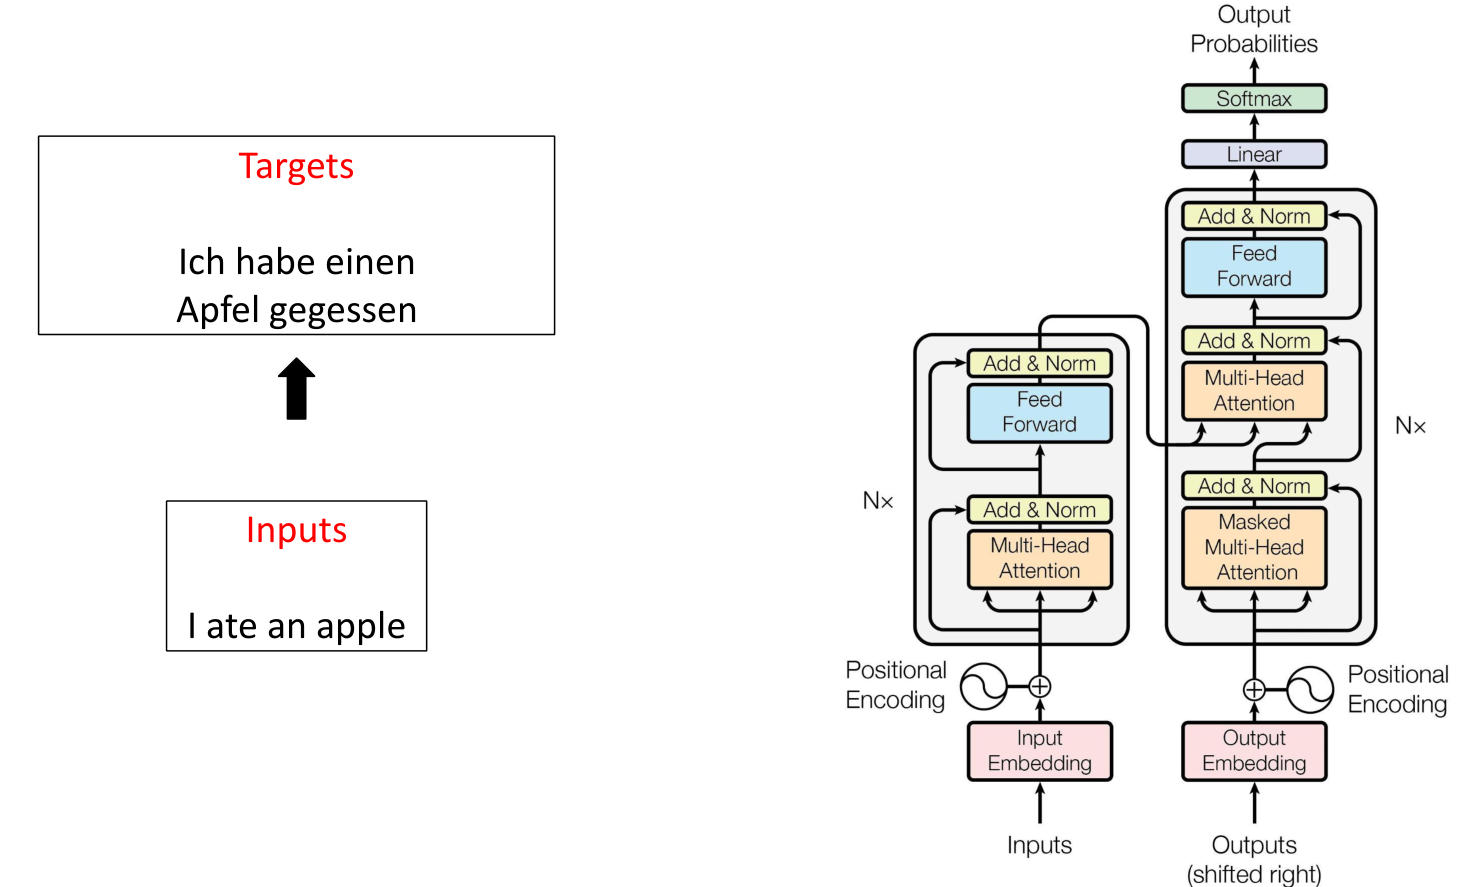
\includegraphics[width=0.8\paperwidth,height=0.8\paperheight,keepaspectratio]{assets/Lecture-6_Introduction_to_Transformers/pdf_page_009.png}
\end{frame}

\begin{frame}{Inputs}
  \centering
  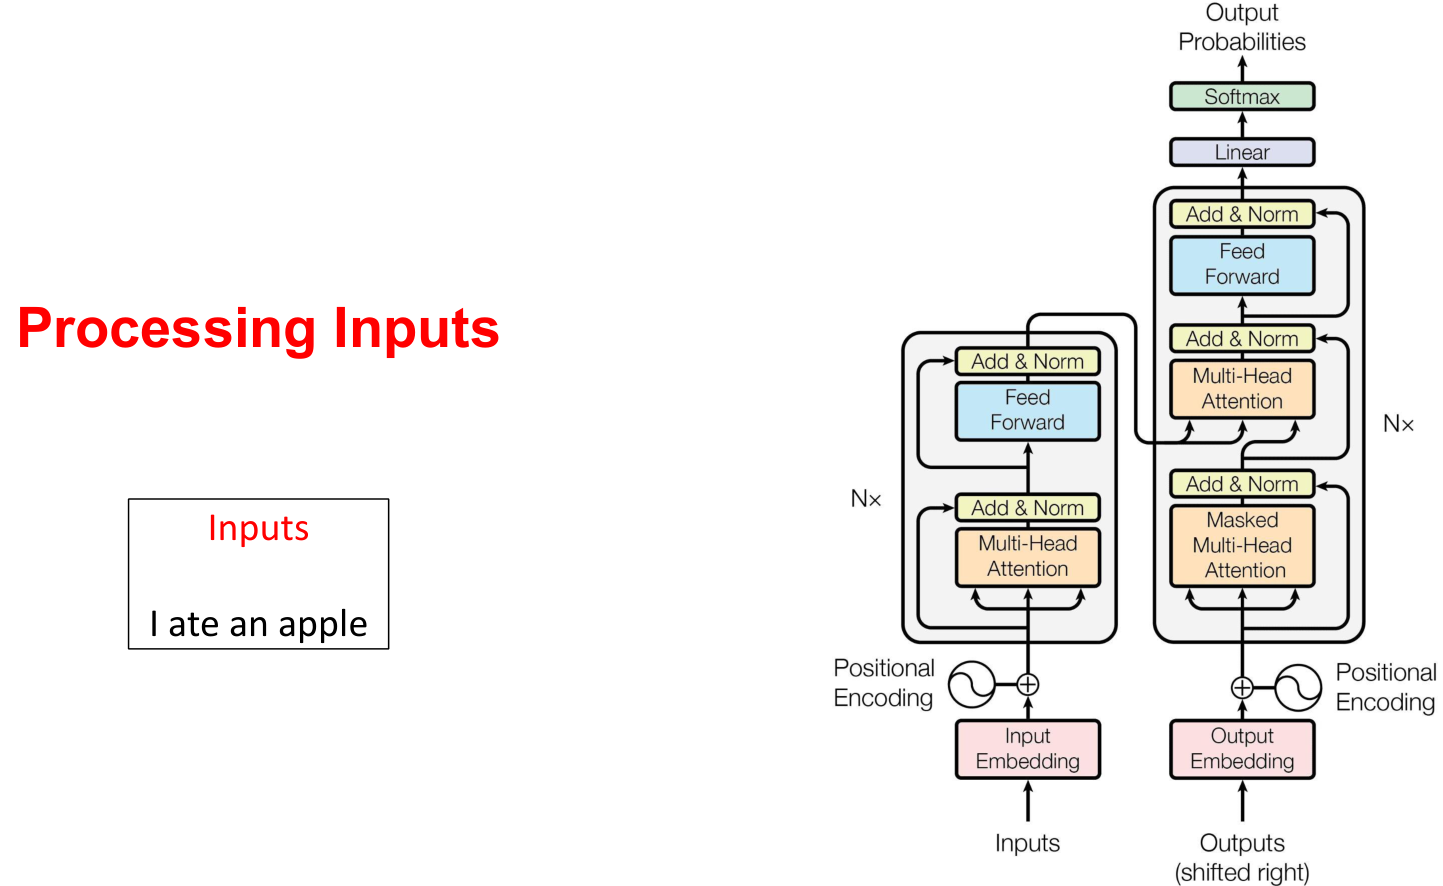
\includegraphics[width=0.8\paperwidth,height=0.8\paperheight,keepaspectratio]{assets/Lecture-6_Introduction_to_Transformers/pdf_page_010.png}
\end{frame}


\begin{frame}{Self-Attention Mechanism}
  \begin{itemize}
    \item[$\blacktriangleright$] Computes contextual representation of a word using all other words
    \item[$\blacktriangleright$] \textbf{Inputs:} Query (Q), Key (K), Value (V)
    \item[$\blacktriangleright$] \textbf{Output:} Weighted sum of values
  \end{itemize}

  \vspace{0.5em}
  \textbf{Attention formula:}
  \begin{align*}
    \text{Attention}(Q, K, V) = \mathrm{softmax}\left(\frac{QK^T}{\sqrt{d_k}}\right)V
  \end{align*}

  \vspace{0.5em}
  \begin{itemize}
    \item[$\blacktriangleright$] Enables each word to attend to all others
  \end{itemize}
\end{frame}

\begin{frame}{Self-Attention Intuition: The ``Bank'' Analogy}
  \begin{itemize}
    \item[$\blacktriangleright$] \textbf{Query:} What we're looking for (e.g., the meaning of ``bank'' in context)
    \item[$\blacktriangleright$] \textbf{Keys:} Tags or features associated with each word/sentence (e.g., ``river'', ``money'')
    \item[$\blacktriangleright$] \textbf{Values:} Information linked to each key (e.g., context-specific meaning)
    \item[$\blacktriangleright$] Uses dot-product similarity between Query and Keys to assign attention weights
    \item[$\blacktriangleright$] Weighted sum of Values produces the contextual representation
  \end{itemize}
\end{frame}

\begin{frame}{Self Attention}
  \centering
  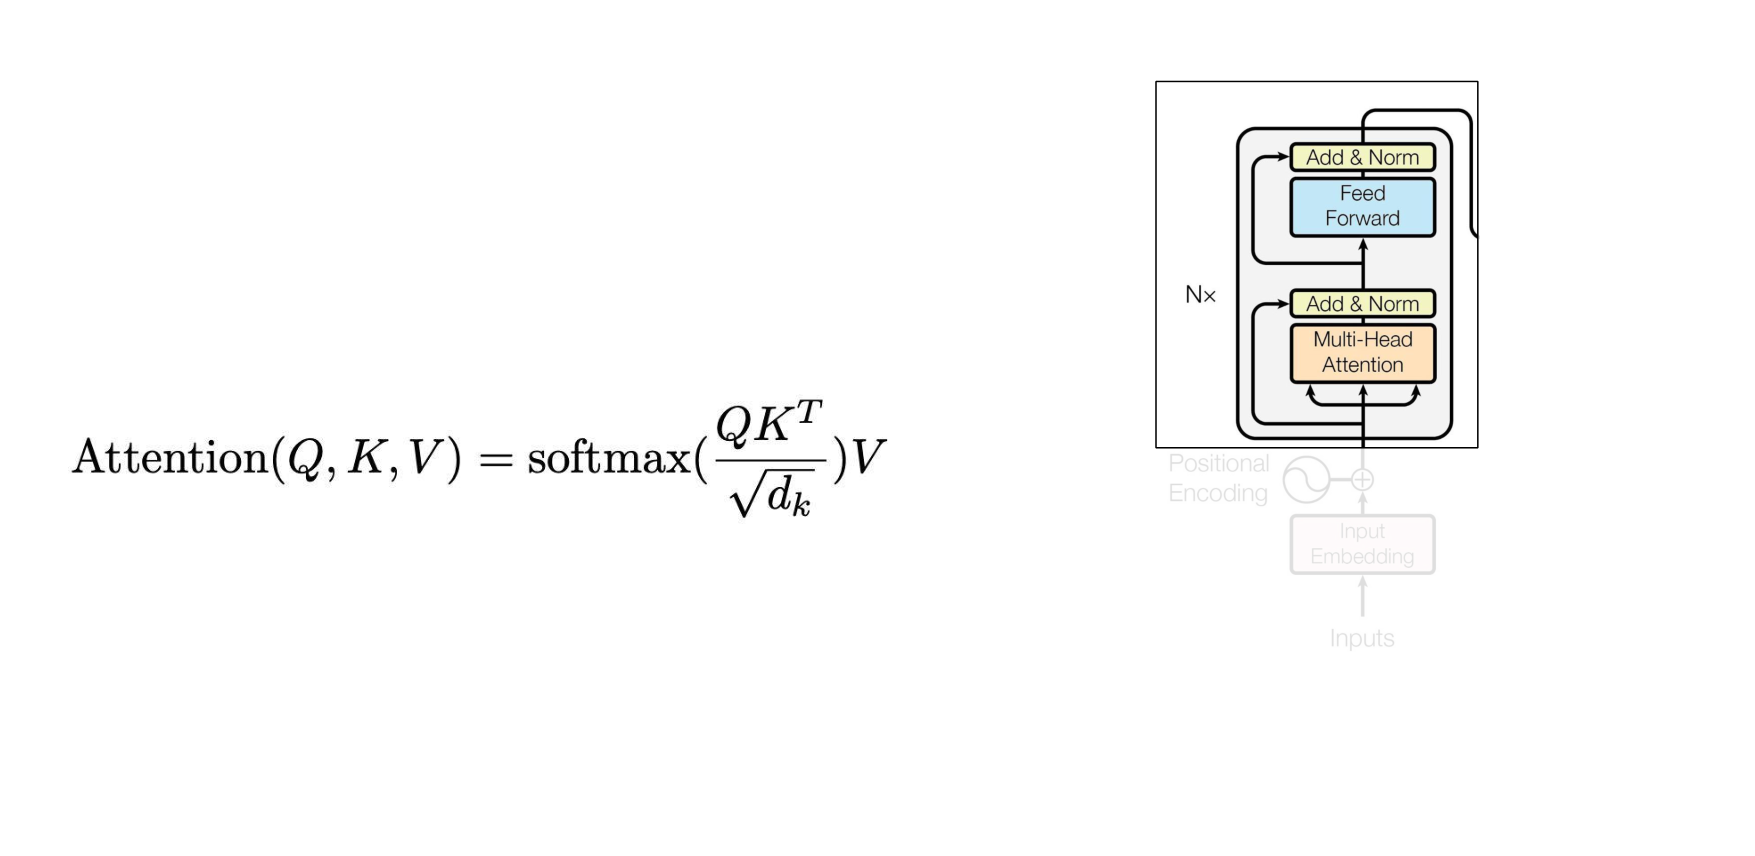
\includegraphics[width=0.9\paperwidth,height=0.95\paperheight,keepaspectratio]{assets/Lecture-6_Introduction_to_Transformers/pdf_page_013.png}
\end{frame}

\begin{frame}{Self Attention}
  \centering
  
\includegraphics[width=0.9\paperwidth,height=0.95\paperheight,keepaspectratio]{assets/Lecture-6_Introduction_to_Transformers/pdf_page_014.png}
\end{frame}

\begin{frame}{Self Attention}
  \centering
  
\includegraphics[width=0.9\paperwidth,height=0.95\paperheight,keepaspectratio]{assets/Lecture-6_Introduction_to_Transformers/pdf_page_015.png}
\end{frame}

\begin{frame}{Self Attention}
  \centering
  
\includegraphics[width=0.9\paperwidth,height=0.95\paperheight,keepaspectratio]{assets/Lecture-6_Introduction_to_Transformers/pdf_page_016.png}
\end{frame}

\begin{frame}{Self Attention}
  \centering
  
\includegraphics[width=0.9\paperwidth,height=0.95\paperheight,keepaspectratio]{assets/Lecture-6_Introduction_to_Transformers/pdf_page_017.png}
\end{frame}

\begin{frame}{Self Attention}
  \centering
  
\includegraphics[width=0.9\paperwidth,height=0.95\paperheight,keepaspectratio]{assets/Lecture-6_Introduction_to_Transformers/pdf_page_018.png}
\end{frame}

\begin{frame}{Self Attention}
  \centering
  
\includegraphics[width=0.9\paperwidth,height=0.95\paperheight,keepaspectratio]{assets/Lecture-6_Introduction_to_Transformers/pdf_page_019.png}
\end{frame}

\begin{frame}{Self Attention}
  \centering
      
\includegraphics[width=0.9\paperwidth,height=0.95\paperheight,keepaspectratio]{assets/Lecture-6_Introduction_to_Transformers/pdf_page_020.png}
\end{frame}

\begin{frame}{Self Attention}
  \centering
  
\includegraphics[width=0.9\paperwidth,height=0.95\paperheight,keepaspectratio]{assets/Lecture-6_Introduction_to_Transformers/pdf_page_021.png}
\end{frame}

\begin{frame}{Self Attention}
  \centering
  
\includegraphics[width=0.9\paperwidth,height=0.95\paperheight,keepaspectratio]{assets/Lecture-6_Introduction_to_Transformers/pdf_page_022.png}
\end{frame}

\begin{frame}{Self Attention}
  \centering
  
\includegraphics[width=0.9\paperwidth,height=0.95\paperheight,keepaspectratio]{assets/Lecture-6_Introduction_to_Transformers/pdf_page_023.png}
\end{frame}

\begin{frame}{Self Attention}
  \centering
  
\includegraphics[width=0.9\paperwidth,height=0.95\paperheight,keepaspectratio]{assets/Lecture-6_Introduction_to_Transformers/pdf_page_024.png}
\end{frame}

\begin{frame}{Self Attention}
  \centering
  
\includegraphics[width=0.9\paperwidth,height=0.95\paperheight,keepaspectratio]{assets/Lecture-6_Introduction_to_Transformers/pdf_page_025.png}
\end{frame}

\begin{frame}{Self Attention}
  \centering
  
\includegraphics[width=0.9\paperwidth,height=0.95\paperheight,keepaspectratio]{assets/Lecture-6_Introduction_to_Transformers/pdf_page_026.png}
\end{frame}

\begin{frame}{Self Attention}
  \centering
  
\includegraphics[width=0.9\paperwidth,height=0.95\paperheight,keepaspectratio]{assets/Lecture-6_Introduction_to_Transformers/pdf_page_027.png}
\end{frame}

\begin{frame}{Self Attention}
  \centering
  
\includegraphics[width=0.9\paperwidth,height=0.95\paperheight,keepaspectratio]{assets/Lecture-6_Introduction_to_Transformers/pdf_page_028.png}
\end{frame}

\begin{frame}{Multi-Head Attention}
  \begin{itemize}
    \item[$\blacktriangleright$] Multi-head attention allows the model to jointly attend to information from different representation subspaces at different positions.
    \item[$\blacktriangleright$] It consists of multiple attention heads, each with its own set of parameters.
    \item[$\blacktriangleright$] The outputs of all heads are concatenated and linearly transformed.
  \end{itemize}

  \vspace{0.7em}

  \textbf{Formula:}
  \[
    \mathrm{MultiHead}(Q, K, V) = \mathrm{Concat}(\text{head}_1, \ldots, \text{head}_h) W^O
  \]
  where each head is defined as:
  \[
    \text{head}_i = \mathrm{Attention}(Q W_i^Q, K W_i^K, V W_i^V)
  \]

  \vspace{0.5em}
  \begin{itemize}
    \item[$\blacktriangleright$] $W_i^Q$, $W_i^K$, and $W_i^V$ are learned projection matrices for each head.
    \item[$\blacktriangleright$] $W^O$ is the output projection matrix that combines the outputs of all heads.
  \end{itemize}
\end{frame}

\begin{frame}{Multi-Head Attention} 
  \centering
  
\includegraphics[width=0.8\paperwidth,height=0.95\paperheight,keepaspectratio]{assets/Lecture-6_Introduction_to_Transformers/pdf_page_030.png}
\end{frame}

\begin{frame}{Multi-Head Attention} 
  \centering
  
\includegraphics[width=0.8\paperwidth,height=0.95\paperheight,keepaspectratio]{assets/Lecture-6_Introduction_to_Transformers/pdf_page_031.png}
\end{frame}

\begin{frame}{Multi-Head Attention} 
  \centering
  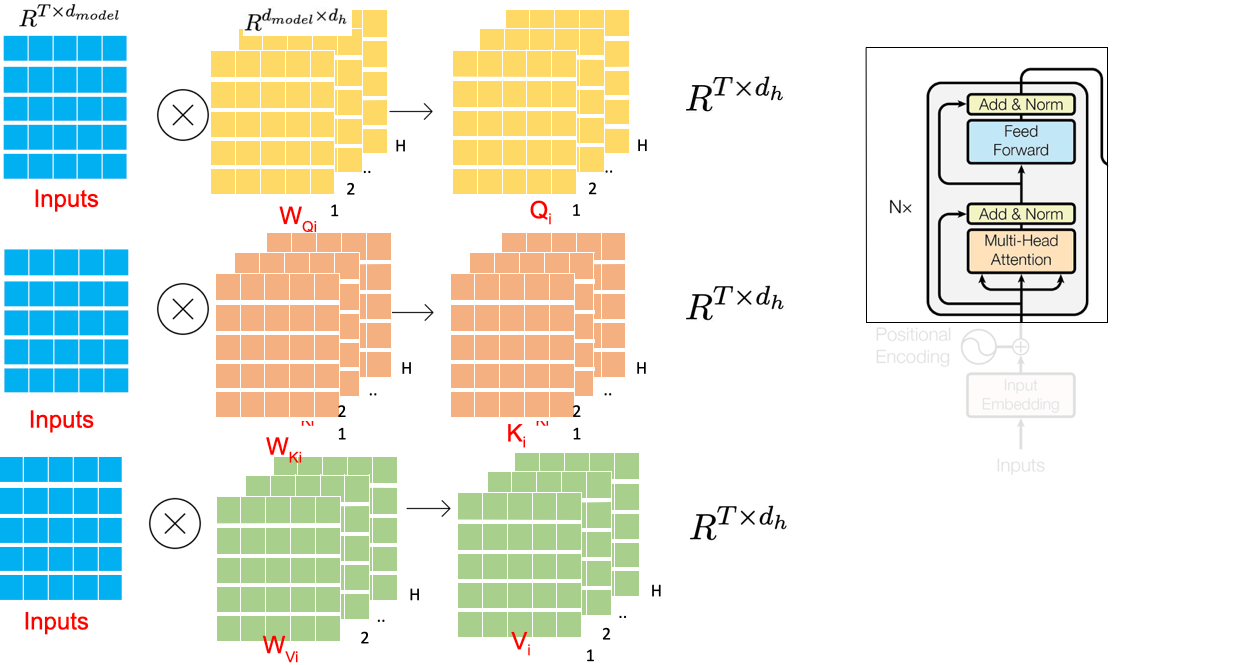
\includegraphics[width=0.8\paperwidth,height=0.95\paperheight,keepaspectratio]{assets/Lecture-6_Introduction_to_Transformers/pdf_page_032.png}
\end{frame}

\begin{frame}{Multi-Head Attention} 
  \centering
  
\includegraphics[width=0.8\paperwidth,height=0.95\paperheight,keepaspectratio]{assets/Lecture-6_Introduction_to_Transformers/pdf_page_033.png}
\end{frame}

\begin{frame}{Multi-Head Attention} 
  \centering
  
\includegraphics[width=0.8\paperwidth,height=0.95\paperheight,keepaspectratio]{assets/Lecture-6_Introduction_to_Transformers/pdf_page_034.png}
\end{frame}

\begin{frame}{Multi-Head Attention} 
  \centering
  
\includegraphics[width=0.8\paperwidth,height=0.95\paperheight,keepaspectratio]{assets/Lecture-6_Introduction_to_Transformers/pdf_page_035.png}
\end{frame}

\begin{frame}{Benefits of Multi-Head Attention}
  \begin{itemize}
    \item[$\blacktriangleright$] Enables the model to jointly attend to information from different representation subspaces at different positions.
    \item[$\blacktriangleright$] Captures various linguistic and syntactic patterns by using multiple attention heads.
    \item[$\blacktriangleright$] Improves the model's ability to represent complex relationships in the data.
    \item[$\blacktriangleright$] Provides richer and more diverse feature representations.
  \end{itemize}
\end{frame}

